\section{Atividade 3}

\subsection{Descrição do Modelo e Análise de Sistema}
Nesta atividade, analisamos um sistema massa-mola-amortecedor, desenvolvendo sua função de transferência com base nos parâmetros especificados. Estes parâmetros são particularmente relevantes para compreender as dinâmicas do sistema:
\begin{itemize}
    \item Massa (\( m \)): 10 kg
    \item Coeficiente de amortecimento (\( C \)): 7 Ns/m
    \item Constante da mola (\( K \)): 5 N/m
\end{itemize}
A função de transferência obtida para o sistema é dada por:
\[
    G(s) = \frac{1}{10s^2 + 7s + 5}
\]

\subsection{Cálculo dos Polos e Parâmetros do Sistema}
Os polos da função de transferência, calculados a partir dos parâmetros do sistema, são:
\begin{itemize}
    \item Polo 1: \( -0.35 + 0.614j \) — indica uma resposta oscilatória amortecida
    \item Polo 2: \( -0.35 - 0.614j \) — complexo conjugado do primeiro polo
\end{itemize}

Os parâmetros do sistema de segunda ordem determinados são:
\begin{itemize}
    \item Frequência natural não-amortecida (\( \omega_n \)): 0.707 rad/s
    \item Coeficiente de amortecimento (\( \zeta \)): 0.495
    \item Ganho estático (\( K_p \)): 0.2
\end{itemize}

\subsection{Resposta ao Impulso}
A resposta ao impulso do sistema foi simulada usando o software Scilab. A figura abaixo mostra como o sistema responde a um impulso aplicado:
\begin{figure}[H]
    \centering
    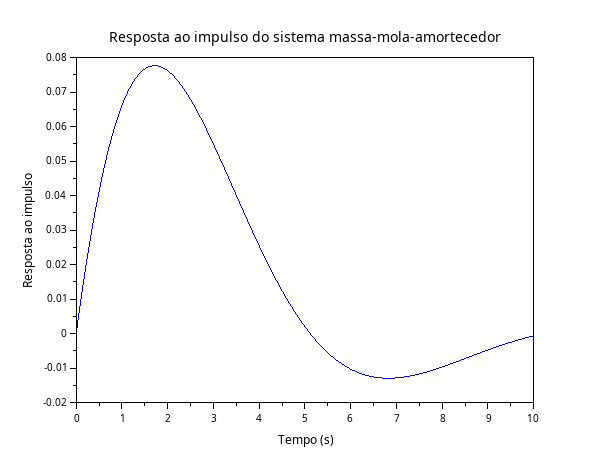
\includegraphics[width=0.8\textwidth]{3-atividade/assets/resposta-ao-impulso.png}
    \caption{Resposta ao impulso do sistema massa-mola-amortecedor}
\end{figure}

\subsection{Discussão}
A análise dos polos confirma que o sistema é subamortecido, evidenciado pelo coeficiente de amortecimento menor que 1. A resposta ao impulso revela um comportamento típico de sistemas subamortecidos: oscilações que decaem com o tempo até a estabilização. O ganho estático (\( K_p \)) reflete a resposta em estado estacionário do sistema a uma entrada de degrau unitário.

\subsection{Conclusões}
Esta atividade proporcionou uma compreensão profunda da influência dos parâmetros físicos — massa, amortecimento e rigidez — na resposta dinâmica de um sistema. Os insights obtidos são cruciais para o design e análise de sistemas de controle adequados para gerenciar tais comportamentos dinâmicos.

